\documentclass[twoside]{article}

\usepackage{aistats2027}
\usepackage[round]{natbib}
\renewcommand{\bibname}{References}
\renewcommand{\bibsection}{\subsubsection*{\bibname}}
\bibliographystyle{apalike}

\usepackage[utf8]{inputenc}
\usepackage[T1]{fontenc}
\usepackage{amsmath,amssymb,amsthm,mathtools}
\usepackage{booktabs}
\usepackage{graphicx}
\usepackage{xcolor}
\usepackage[hidelinks]{hyperref}
\usepackage{cleveref}
\usepackage{enumitem}
\usepackage{seqsplit}

\newtheorem{theorem}{Theorem}
\newtheorem{proposition}[theorem]{Proposition}
\newtheorem{lemma}[theorem]{Lemma}
\newtheorem{corollary}[theorem]{Corollary}
\theoremstyle{definition}
\newtheorem{definition}[theorem]{Definition}
\theoremstyle{remark}
\newtheorem{remark}[theorem]{Remark}

\newcommand{\E}{\mathbb{E}}
\newcommand{\R}{\mathbb{R}}
\newcommand{\tr}{\operatorname{tr}}
\newcommand{\corr}{\operatorname{corr}}
\newcommand{\cka}{\operatorname{CKA}}
\newcommand{\deff}{d_{\mathrm{eff}}}
\newcommand{\Srho}{S_{\rho}}

\newcommand{\SynMAE}{0.010}
\newcommand{\SynCorr}{0.999}
\newcommand{\SynCKAMAE}{0.37}
\newcommand{\SynCKACorr}{0.32}
\newcommand{\SynCKAMAEsmall}{0.57}
\newcommand{\SynCKAMAElarge}{0.07}
\newcommand{\SynHighCKA}{0.998}
\newcommand{\SynHighCKAEU}{0.06}
\newcommand{\SynLowCKA}{0.003}
\newcommand{\SynLowCKAEU}{0.96}
\newcommand{\SynSameOne}{0.76}
\newcommand{\SynSameOneTheory}{0.86}
\newcommand{\CeilingCIFARh}{0.70}
\newcommand{\CeilingCI}{0.69--0.71}
\newcommand{\EntropyDirichlet}{0.95}
\newcommand{\GateMin}{0.89}
\newcommand{\GateMax}{0.96}
\newcommand{\EtwoFracTenMean}{0.90}
\newcommand{\EtwoFracTenPartialMean}{0.26}
\newcommand{\EtwoRetestMean}{1.00}
\newcommand{\EtwoHalvesMean}{0.91}
\newcommand{\EtwoAUFracTenMean}{0.90}
\newcommand{\EtwoFalsA}{not triggered}
\newcommand{\EtwoDropEU}{0.10}
\newcommand{\EtwoDropAU}{0.10}
\newcommand{\EtwoRetEU}{46\%}
\newcommand{\EtwoRetAU}{53\%}
\newcommand{\EtwoRetestPartial}{0.56}
\newcommand{\EtwoAURetestPartial}{0.87}
\newcommand{\EtwoAUFracTenPartial}{0.46}
\newcommand{\EtwoMIFracTenPartial}{0.37}
\newcommand{\EtwoMIRetestPartial}{0.76}
\newcommand{\EtwoHalvesPartial}{0.36}
\newcommand{\EtwoFalsB}{\textbf{triggered}}
\newcommand{\AUHumanMin}{0.34}
\newcommand{\AUHumanMax}{0.43}
\newcommand{\AUHumanNormMin}{0.40}
\newcommand{\AUHumanNormMax}{0.51}
\newcommand{\SqrtCeiling}{0.84}
\newcommand{\AUHumanRangeMax}{0.05}
\newcommand{\EtwobScaleText}{At fixed weight decay, EU moves with $c$: across $c\in[0.1,10]$ the mean Laplace logit variance changes by a factor between 0.017 and 61.7, the mean bootstrap width between 0.38 and 1.84, and EU rankings change (Laplace MI rank agreement down to 0.72, bootstrap width down to 0.89). When the weight decay is re-tuned by validation, the selected value scales as $c^2$ (from $10^{-5}$ at $c=0.1$ to $10^{-1}$ at $c=10$), which is exactly the prior change of \Cref{prop:scale}, and the largest deviation of any EU rank agreement or mean ratio from the untransformed head is 0.086 (the re-tuned grid is coarse, one decade per step).}
\newcommand{\EtwobTailCKAMin}{0.956}
\newcommand{\EtwobTailMKNNMin}{0.62}
\newcommand{\EtwobTailLapMax}{2.3}
\newcommand{\EtwobTailWidthMax}{1.39}
\newcommand{\EtwobTailBLRdev}{0.04}
\newcommand{\EtwobBootLessLaplace}{6 of 6}
\newcommand{\SrhoVsEUwidth}{0.87}
\newcommand{\SrhoVsEUblr}{0.92}
\newcommand{\CKAVsEUwidth}{0.66}
\newcommand{\CKAVsEUblr}{0.76}
\newcommand{\MKNNVsEUwidth}{0.85}
\newcommand{\MKNNVsEUblr}{0.90}
\newcommand{\RealThmMAE}{0.34}
\newcommand{\RealThmRank}{0.93}
\newcommand{\RealThmRankCKA}{0.74}
\newcommand{\SrhoVsEUwidthPartial}{0.83}
\newcommand{\CKAVsEUwidthPartial}{0.64}
\newcommand{\MKNNVsEUwidthPartial}{0.72}
\newcommand{\SrhoVsAU}{0.92}
\newcommand{\CrossEncPartial}{0.10}
\newcommand{\HighCKAPartial}{0.21}
\newcommand{\SrhoFals}{not triggered}
\newcommand{\DeffVsBLR}{0.90}
\newcommand{\DeffVsWidth}{-0.19}
\newcommand{\PRVsWidth}{-0.64}
\newcommand{\EfourCKA}{0.837}
\newcommand{\EfourRep}{93\%}
\newcommand{\EfourHead}{-2\%}
\newcommand{\EfourData}{9\%}
\newcommand{\EfourFloor}{0.00}
\newcommand{\PreregHash}{05aa7d680e7d7f11\ldots}
\newcommand{\PreregHashFull}{\seqsplit{05aa7d680e7d7f11ec6ccca283c8c56ddf021a971ae97de23d94528935d3cc70}}
\newcommand{\ResolventWorst}{4.97}
\newcommand{\Mens}{50}
\newcommand{\MChoice}{M-stability (DINOv2-B, final layer): Spearman between independent ensembles of size $M$ and $2M$: $M=10$: 0.992, $M=25$: 0.997, $M=50$: 0.998, $M=100$: 0.999. We use $M=50$.}
\newcommand{\EfourPRep}{61\%}
\newcommand{\EfourPHead}{10\%}
\newcommand{\EfourPData}{30\%}
\newcommand{\EfourPFloor}{0.33}
\newcommand{\LOEOdiffCKAmin}{0.09}
\newcommand{\LOEOdiffCKAmax}{0.26}
\newcommand{\LOEOdiffCKApos}{5}
\newcommand{\LOEOdiffCKAblrPos}{4}
\newcommand{\LOEOdiffLinMin}{-0.08}
\newcommand{\LOEOdiffLinMax}{+0.05}
\newcommand{\LOEOdiffMknnMin}{-0.04}
\newcommand{\LOEOdiffMknnMax}{+0.17}
\newcommand{\CBdiffCKA}{0.19}
\newcommand{\LinVsEUwidthPartial}{0.83}
\newcommand{\LinVsEUwidth}{0.41}
\newcommand{\SzeroVsEUwidthPartial}{0.83}
\newcommand{\SweepLOEOposBLR}{5}
\newcommand{\SweepLOEOposW}{5}
\newcommand{\CorrWidthConfMax}{-0.997}
\newcommand{\CorrWidthConfMin}{-0.999}
\newcommand{\CorrWidthAUMin}{0.994}
\newcommand{\CorrWidthBLRMin}{-0.08}
\newcommand{\CorrWidthBLRMax}{0.31}
\newcommand{\McurveWten}{0.45}
\newcommand{\McurveWfifty}{0.60}
\newcommand{\McurveWtwohundred}{0.82}
\newcommand{\McurveMItwohundred}{0.90}
\newcommand{\RdFracW}{0.27}
\newcommand{\RdFracWsd}{0.10}
\newcommand{\RdFracWTop}{0.70}
\newcommand{\RdFracWCorr}{0.48}
\newcommand{\RdFracWCorrMin}{0.26}
\newcommand{\RdFracWCorrMax}{0.66}
\newcommand{\RdFracAU}{0.46}
\newcommand{\RdFracAUsd}{0.11}
\newcommand{\RdFracAUTop}{0.72}
\newcommand{\RdFracAUCorr}{0.52}
\newcommand{\RdFracAUCorrMin}{0.42}
\newcommand{\RdFracAUCorrMax}{0.65}
\newcommand{\RdFracMI}{0.39}
\newcommand{\RdFracMIsd}{0.04}
\newcommand{\RdFracMITop}{0.70}
\newcommand{\RdFracMICorr}{0.50}
\newcommand{\RdFracMICorrMin}{0.42}
\newcommand{\RdFracMICorrMax}{0.57}
\newcommand{\RdHalfW}{0.36}
\newcommand{\RdHalfWsd}{0.08}
\newcommand{\RdHalfWTop}{0.72}
\newcommand{\RdHalfWCorr}{0.68}
\newcommand{\RdHalfWCorrMin}{0.50}
\newcommand{\RdHalfWCorrMax}{0.79}
\newcommand{\RdHalfAU}{0.53}
\newcommand{\RdHalfAUsd}{0.08}
\newcommand{\RdHalfAUTop}{0.74}
\newcommand{\RdHalfAUCorr}{0.61}
\newcommand{\RdHalfAUCorrMin}{0.53}
\newcommand{\RdHalfAUCorrMax}{0.69}
\newcommand{\RdHalfMI}{0.52}
\newcommand{\RdHalfMIsd}{0.05}
\newcommand{\RdHalfMITop}{0.73}
\newcommand{\RdHalfMICorr}{0.70}
\newcommand{\RdHalfMICorrMin}{0.63}
\newcommand{\RdHalfMICorrMax}{0.76}
\newcommand{\RdRetestW}{0.56}
\newcommand{\RdRetestWsd}{0.03}
\newcommand{\RdRetestWTop}{0.93}
\newcommand{\RdRetestAU}{0.87}
\newcommand{\RdRetestAUsd}{0.10}
\newcommand{\RdRetestAUTop}{0.97}
\newcommand{\RdRetestMI}{0.76}
\newcommand{\RdRetestMIsd}{0.03}
\newcommand{\RdRetestMITop}{0.90}
\newcommand{\SensMaxDiff}{0.001}
\newcommand{\RdDraws}{3}
\newcommand{\SweepWdMax}{1}
\newcommand{\SweepDeffMin}{0.06}
\newcommand{\SweepDeffMax}{0.29}
\newcommand{\SweepAccMin}{0.50}
\newcommand{\SweepAccMax}{0.97}
\newcommand{\SweepBLRsrho}{0.94}
\newcommand{\SweepBLRszero}{0.89}
\newcommand{\SweepBLRcka}{0.69}
\newcommand{\SweepWsrho}{0.96}
\newcommand{\SweepWszero}{0.88}
\newcommand{\SweepWcka}{0.71}
\newcommand{\SweepTrainOnlyMaxDiff}{0.03}
\newcommand{\SweepBLRsrhoMinusSzeroMax}{0.05}
\newcommand{\SweepWsrhoMinusSzeroMax}{0.08}
\newcommand{\SweepDiffBLR}{+0.05}
\newcommand{\SweepDiffBLRlo}{-0.01}
\newcommand{\SweepDiffBLRhi}{+0.13}
\newcommand{\SweepDiffSmallBLR}{-0.02}
\newcommand{\SweepDiffW}{+0.08}
\newcommand{\SweepDiffWlo}{+0.00}
\newcommand{\SweepDiffWhi}{+0.13}
\newcommand{\SweepDiffSmallW}{+0.05}
\newcommand{\CrossTopTen}{0.38}
\newcommand{\GaussMAEreal}{0.34}
\newcommand{\GaussMAEgauss}{0.019}
\newcommand{\RhoEffMed}{0.12}
\newcommand{\RhoEffMin}{0.003}
\newcommand{\RhoEffMax}{0.52}
\newcommand{\RhoEffRatioMed}{120}
\newcommand{\SrhoEffVsEUwidthPartial}{0.78}
\newcommand{\SrhoEffVsEUblr}{0.93}
\newcommand{\RhoEffText}{its curvature-calibrated prior strength $\rho_{\mathrm{eff}}=\mathrm{wd}/\bar h$, with $\bar h$ the mean $p(1-p)$ of the MAP head, is a median 120 times larger}
\newcommand{\MtwoEncs}{5}
\newcommand{\MtFracW}{0.34}
\newcommand{\MtFracWCorr}{0.43}
\newcommand{\MtFracWCorrLo}{0.20}
\newcommand{\MtFracWCorrHi}{0.58}
\newcommand{\MtFracAU}{0.45}
\newcommand{\MtFracAUCorr}{0.48}
\newcommand{\MtFracAUCorrLo}{0.30}
\newcommand{\MtFracAUCorrHi}{0.65}
\newcommand{\MtFracMI}{0.47}
\newcommand{\MtFracMICorr}{0.52}
\newcommand{\MtFracMICorrLo}{0.42}
\newcommand{\MtFracMICorrHi}{0.60}
\newcommand{\MtHalfW}{0.47}
\newcommand{\MtHalfWCorr}{0.63}
\newcommand{\MtHalfWCorrLo}{0.44}
\newcommand{\MtHalfWCorrHi}{0.79}
\newcommand{\MtHalfAU}{0.53}
\newcommand{\MtHalfAUCorr}{0.57}
\newcommand{\MtHalfAUCorrLo}{0.42}
\newcommand{\MtHalfAUCorrHi}{0.70}
\newcommand{\MtHalfMI}{0.65}
\newcommand{\MtHalfMICorr}{0.73}
\newcommand{\MtHalfMICorrLo}{0.65}
\newcommand{\MtHalfMICorrHi}{0.80}
\newcommand{\MtRetestW}{0.79}
\newcommand{\MtRetestAU}{0.94}
\newcommand{\MtRetestMI}{0.90}
\newcommand{\MtWdDivW}{0.35}
\newcommand{\MtWdDivWCorr}{0.42}
\newcommand{\MtWdDivWCorrLo}{0.15}
\newcommand{\MtWdDivWCorrHi}{0.87}
\newcommand{\MtWdDivAU}{0.29}
\newcommand{\MtWdDivAUCorr}{0.31}
\newcommand{\MtWdDivAUCorrLo}{-0.05}
\newcommand{\MtWdDivAUCorrHi}{0.90}
\newcommand{\MtWdDivMI}{0.38}
\newcommand{\MtWdDivMICorr}{0.44}
\newcommand{\MtWdDivMICorrLo}{0.04}
\newcommand{\MtWdDivMICorrHi}{0.93}
\newcommand{\MtWdMulW}{0.63}
\newcommand{\MtWdMulWCorr}{0.74}
\newcommand{\MtWdMulWCorrLo}{0.53}
\newcommand{\MtWdMulWCorrHi}{0.84}
\newcommand{\MtWdMulAU}{0.57}
\newcommand{\MtWdMulAUCorr}{0.59}
\newcommand{\MtWdMulAUCorrLo}{0.23}
\newcommand{\MtWdMulAUCorrHi}{0.81}
\newcommand{\MtWdMulMI}{0.62}
\newcommand{\MtWdMulMICorr}{0.68}
\newcommand{\MtWdMulMICorrLo}{0.40}
\newcommand{\MtWdMulMICorrHi}{0.87}
\newcommand{\ResidFracMin}{0.2\%}
\newcommand{\ResidFracMax}{0.6\%}
\newcommand{\ResidFracAUMax}{0.7\%}
\newcommand{\MtCIbelowOne}{100\%}


\begin{document}

\twocolumn[
\aistatstitle{When Do Aligned Representations Agree on What They Do Not Know? \\ CKA, Prior Strength and the Spectral Tail}
\aistatsauthor{Anonymous Authors}
\aistatsaddress{Anonymous Institution}
]

\begin{abstract}
Representational alignment, measured by mutual nearest neighbours in the platonic-representation literature and by centred kernel alignment (CKA) more broadly, is the main evidence that different vision models learn similar representations.
We ask when linear heads on two encoders agree about \emph{what they do not know}, and show that high CKA does not imply it, for two reasons we make exact.
For Bayesian linear heads on Gaussian features, the correlation across inputs of two heads' epistemic variances equals a ridge-regularised alignment index $\Srho$ at the heads' own prior strength.
CKA is the $\rho\to\infty$ limit of this index and weights spectral directions by squared variance, whereas epistemic uncertainty (EU) counts every direction above $\rho$; we construct pairs with CKA $>0.99$ and EU correlation $0.06$, and the converse.
CKA is also blind to feature scale, which acts on EU as a change of prior; so are whitened indices, and only $\Srho$ evaluated at the head's prior strength on the head's own feature scaling is not.
Representation-only non-identification follows already from the dependence of EU on prior and data; our results say \emph{which} spectral information an index needs and predict that whitened, canonical-correlation-type indices should outperform CKA for weakly regularised heads.
On five frozen encoders with CIFAR-10H labels, the evidence is consistent with this but limited: across 30 encoder pairs, $\Srho$, its CCA-type limit and linear predictivity order confidence-controlled EU agreement at Spearman $\approx$\SrhoVsEUwidthPartial{} against \CKAVsEUwidthPartial{} for CKA, the advantage over CKA is positive whichever encoder is left out (\LOEOdiffCKAmin{} to \LOEOdiffCKAmax{}), but with five encoders no valid sampling interval exists, and no index beats linear predictivity or mutual $k$-NN.
Heads on identical features (CKA $=1$) trained on different data disagree, and rescaling features at fixed weight decay shifts mean Laplace EU over three orders of magnitude while CKA stays at one.
For softmax probes, EU summaries are almost a function of confidence (rank correlation \CorrWidthConfMin{} to \CorrWidthConfMax{}), so EU and aleatoric agreement behave alike; this and other failed pre-registered predictions are reported in full.
\end{abstract}

\section{INTRODUCTION}

Neural networks trained with different objectives, architectures and data are converging toward similar representations; the platonic-representation hypothesis rests mainly on mutual nearest-neighbour overlap and its growth with model scale \citep{huh2024platonic}, and the broader literature uses centred kernel alignment \citep[CKA;][]{kornblith2019similarity} and canonical correlations \citep{raghu2017svcca,morcos2018insights}.
A natural but untested inference is that aligned encoders also induce heads that are unsure about the same inputs, which would make alignment a label-free tool for transferring uncertainty estimates, selecting encoders for active learning, or arguing that aligned models share blind spots.
We are not aware of work that uses alignment this way explicitly; our question is whether doing so would be justified.

We study this for \emph{epistemic} uncertainty (EU), the reducible part that reflects limited data \citep{kendall2017uncertainties,hullermeier2021aleatoric}.
At one level the answer is immediate: the EU of a head depends on its prior and training data, which no function of two representations can see.
The useful question is sharper: \emph{which} information about a pair of representations controls EU agreement once the head is fixed, and do the common indices carry it?
For CKA our answer is no: it discards two pieces of information that matter.
It normalises away the scale of the features, and a regularised head treats scale as part of its prior.
And it weights spectral directions by their squared variance, whereas EU counts every direction above the regularisation level, however small its variance.

\paragraph{Contributions.}
\begin{enumerate}[leftmargin=*,itemsep=1pt,topsep=1pt]
\item \textbf{An exact identity} (\Cref{thm:identity}): for Gaussian features and Bayesian linear heads, the correlation of two heads' epistemic variances equals $\Srho$, the cosine between ridge smoothers at the heads' prior strengths, an index from the ridge-CCA family. CKA is its $\rho\to\infty$ limit and a normalised sum of squared canonical correlations its $\rho\to0$ limit (\Cref{prop:limits}).
\item \textbf{Why CKA fails}: CKA is neither necessary nor sufficient for EU agreement (\Cref{cor:neither}); its invariances are not invariances of EU (\Cref{prop:scale,prop:tail}); and even identical features give imperfect EU agreement once priors differ (\Cref{cor:same}). Supporting results (\Cref{prop:resolvent,lem:deff,lem:boot}) are elementary or classical and stated for completeness.
\item \textbf{Pre-registered and additional exploratory experiments} on five frozen encoders with CIFAR-10H human labels, using bootstrap, Laplace and closed-form estimators, re-test reliabilities, leave-one-encoder-out sensitivity analyses and reliability ceilings. Confirmed and failed predictions are reported alike (\Cref{tab:prereg}).
\end{enumerate}

\section{SETUP AND RELATED WORK}
\label{sec:setup}

\paragraph{Representations and alignment.}
An encoder $\phi_A:\mathcal X\to\R^{d_A}$ is frozen; inputs $x\sim P$.
We centre features and write $\Sigma_A=\E[\phi_A\phi_A^\top]$, $\Sigma_{AB}=\E[\phi_A\phi_B^\top]$.
Population linear CKA is $\cka(A,B)=\|\Sigma_{AB}\|_F^2/(\|\Sigma_A\|_F\|\Sigma_B\|_F)$ \citep{kornblith2019similarity}; it is invariant to $\phi\mapsto cQ\phi$ for $c>0$ and orthogonal $Q$.
Mutual $k$-NN with cosine similarity \citep{huh2024platonic} shares this invariance.
Prior work has already shown that CKA can miss functionally relevant differences: it is insensitive to low-variance directions that matter for downstream behaviour \citep{ding2021grounding} and can be manipulated without changing function \citep{davari2023reliability}. Our tail argument is a special case of this insensitivity, made exact for one downstream quantity. Other lines of work regularise shape metrics \citep{williams2021generalized}, define distances through ridge-regularised linear prediction \citep[GULP;][]{boixadsera2022gulp}, or interpret CKA and CCA as average alignment of optimal linear decoders \citep{harvey2024decodable}; see also RSA \citep{kriegeskorte2008rsa}. These works concern predictions or decodable information, and error consistency compares which items two models get wrong \citep{geirhos2020error}. We ask what alignment implies for the \emph{uncertainty} of a head. Human soft labels are used here only as an evaluation target; on learning from annotator disagreement see \citet{uma2021disagreement}.

\paragraph{Heads and epistemic uncertainty.}
A head is fitted on $n$ labelled examples with feature matrix $\Phi_A\in\R^{n\times d_A}$.
For a Bayesian linear head with prior $w\sim\mathcal N(0,\tau^2 I)$ and noise variance $\sigma^2$, the posterior variance of $w^\top\phi_A(x)$ is
\begin{equation}
v_A(x)=\sigma^2\phi_A(x)^\top(\Phi_A^\top\Phi_A+\lambda I)^{-1}\phi_A(x),\quad \lambda=\sigma^2/\tau^2,
\label{eq:blr}
\end{equation}
which does not depend on the labels \citep{rasmussen2006gpml}.
With $\hat\Sigma_A=\Phi_A^\top\Phi_A/n$ and $\rho=\lambda/n$, $n v_A(x)/\sigma^2=\phi_A(x)^\top(\hat\Sigma_A+\rho I)^{-1}\phi_A(x)$.
We call the population version $u_A(x)=\phi_A(x)^\top(\Sigma_A+\rho_A I)^{-1}\phi_A(x)$ the \emph{EU score}; it is the ridge leverage score of $x$ \citep{alaoui2015ridge}, whose average over the training points is the effective dimension, and interpolates between a Mahalanobis leverage ($\rho\to0$) and a squared norm ($\rho\to\infty$), connecting to Bayesian last-layer and neural-linear models \citep{snoek2015scalable,riquelme2018showdown} and to distance-aware feature-space uncertainty \citep{lee2018mahalanobis,vanamersfoort2020duq,liu2020sngp,mukhoti2023ddu}.
In experiments we also use softmax heads with bootstrap ensembles \citep{efron1993bootstrap,lakshminarayanan2017ensembles}, summarised by the mutual information \citep{houlsby2011bald} and by quantile-interval widths, and last-layer Laplace \citep{daxberger2021laplace}.
Entropy-based decompositions have known limitations \citep{wimmer2023quantifying}, and in practice AU and EU estimators are strongly entangled \citep{mucsanyi2024benchmarking}; we therefore report several EU summaries, including the closed form, which does not depend on labels.

\paragraph{EU agreement.}
For two models we measure agreement as the correlation of their EU scores across inputs; in experiments, as Spearman correlation, partial Spearman controlling for both models' confidence and human-label entropy, and Spearman within human-entropy deciles.
Partial and stratified variants reduce, but cannot remove, the trivial explanation that both models are uncertain on intrinsically ambiguous images, because human entropy is itself a noisy covariate (reliability \CeilingCIFARh{}); \Cref{sec:e2} reports a sensitivity analysis over covariate estimators.

\section{THEORY}
\label{sec:theory}

All proofs are in \Cref{app:proofs}. Let $w_i(\rho)=\lambda_i/(\lambda_i+\rho)$ for eigenvalues $\lambda_i$ of a covariance.

\begin{definition}[Spectral agreement index]
For symmetric $M_A,M_B$ let
\[
S(M_A,M_B)=\frac{\tr(M_A\Sigma_{AB}M_B\Sigma_{BA})}{\sqrt{\tr\big((M_A\Sigma_A)^2\big)\,\tr\big((M_B\Sigma_B)^2\big)}},
\]
and $\Srho:=S\big((\Sigma_A+\rho_A I)^{-1},(\Sigma_B+\rho_B I)^{-1}\big)$.
\end{definition}
On a sample, $\Srho$ is the Frobenius cosine between the ridge smoothers $H=\Phi(\Phi^\top\Phi+n\rho I)^{-1}\Phi^\top$, computable with $d\times d$ matrices only.
$\Srho$ is not a new similarity measure: ridge interpolation between correlation and covariance analyses is classical \citep{vinod1976canonical,bach2002kernelica}, and GULP \citep{boixadsera2022gulp} compares representations through ridge-regularised linear predictors, which is closely related. Comparisons of optimal linear readouts also underlie CKA and CCA \citep{harvey2024decodable}. What we add is the exact link between this family and agreement of \emph{posterior variances}, which identifies the head's own prior strength as the right regularisation level.

\begin{theorem}[EU agreement identity]
\label{thm:identity}
If $(\phi_A(x),\phi_B(x))$ is zero-mean jointly Gaussian under $x\sim P$, then for any symmetric $M_A,M_B$,
$\corr\big(\phi_A^\top M_A\phi_A,\;\phi_B^\top M_B\phi_B\big)=S(M_A,M_B)$.
In particular $\corr(u_A,u_B)=\Srho$.
\end{theorem}

\begin{proposition}[Limits]
\label{prop:limits}
With $\rho_A=\rho_B=\rho$: (i) $\lim_{\rho\to\infty}\Srho=\cka(A,B)$; (ii) if $\Sigma_A,\Sigma_B$ are invertible, $\lim_{\rho\to 0}\Srho=\sum_j r_j^2/\sqrt{d_Ad_B}$, where $r_j$ are the canonical correlations of $A$ and $B$; for $d_A=d_B=d$ this is the mean squared canonical correlation (the $R^2_{\mathrm{CCA}}$ similarity), and otherwise the sum of squared canonical correlations normalised by $\sqrt{d_Ad_B}$.
\end{proposition}

The proof is one application of Isserlis' theorem; its value lies in the interpretation.
\citet{kornblith2019similarity} already observed that CCA, linear regression and CKA differ in how they weight eigendirections; what the identity adds is the weighting that EU agreement requires. In the eigenbasis, CKA weighs a shared direction by $\lambda_i^2$, whereas $\Srho$ weighs it by $w_i(\rho)^2$: every direction with $\lambda_i\gg\rho$ counts as one, however small its variance.
This gives a concrete prediction: when heads are weakly regularised, whitened (CCA-type) indices should track EU agreement better than CKA, reversing the preference for CKA over CCA that \citet{kornblith2019similarity} established for a different target (identifying corresponding layers).
Since learned representations have long, power-law spectral tails \citep{agrawal2022alphareq}, as do population codes in visual cortex \citep{stringer2019highdim}, the two indices read different parts of the spectrum.
Mutual $k$-NN with cosine similarity sits in between: like CKA it is invariant to $cQ$, so it is blind to scale, but as a local, rank-based statistic it is not dominated by the top eigendirections and responds to the tail (it drops to \EtwobTailMKNNMin{} under the tail reshaping of \Cref{sec:e2b}, where CKA stays above \EtwobTailCKAMin{}).

\begin{corollary}[CKA is neither necessary nor sufficient]
\label{cor:neither}
Let $\phi_A=(s,a)$, $\phi_B=(s,b)$ with $s\in\R^k$, $a,b\in\R^m$ independent Gaussians with covariances $\lambda_s I,\lambda_pI,\lambda_pI$. Then
$\cka=\frac{k\lambda_s^2}{k\lambda_s^2+m\lambda_p^2}$ and
$\corr(u_A,u_B)=\frac{k w_s^2}{k w_s^2+m w_p^2}$.
Hence for every $\epsilon>0$ there are pairs with $\cka\ge 1-\epsilon$ and $\corr(u_A,u_B)\le\epsilon$, and pairs with $\cka\le\epsilon$ and $\corr(u_A,u_B)\ge1-\epsilon$.
\end{corollary}

\begin{proposition}[Scale is a prior change]
\label{prop:scale}
For $c>0$ and orthogonal $Q$, $\cka(\phi,cQ\phi)=1$, cosine $k$-NN graphs are unchanged, and $v(cQ\Phi,cQx;\lambda)=v(\Phi,x;\lambda/c^2)$.
Under Gaussian features, the EU agreement between the head on $cQ\phi$ and the head on $\phi$ at the same $\lambda$ is
$\sum_i w_i(\rho)w_i(\rho/c^2)\big/\sqrt{\sum_i w_i(\rho)^2\sum_i w_i(\rho/c^2)^2}$, which is $<1$ unless the spectrum is flat on its support.
\end{proposition}

\begin{proposition}[Tail reshaping]
\label{prop:tail}
Let $\Sigma=U\Lambda U^\top$, let $\mathcal T$ be a set of tail directions, and let $T_s$ scale them by $s$.
With $\eta=\sum_{i\in\mathcal T}\lambda_i^2/\sum_{i\notin\mathcal T}\lambda_i^2$,
$\cka(\phi,T_s\phi)=\frac{1+s^2\eta}{\sqrt{(1+\eta)(1+s^4\eta)}}\ge 1-(s^2-1)^2\eta$,
whereas the effective dimension changes by $\sum_{i\in\mathcal T}\big[w_i(\rho/s^2)-w_i(\rho)\big]$.
\end{proposition}

\begin{lemma}[Mean EU is effective dimension]
\label{lem:deff}
On the training points, $\frac1n\sum_{i}v(x_i)=\frac{\sigma^2}{n}\deff(\rho)$ with $\deff(\rho)=\sum_i\frac{\hat\lambda_i}{\hat\lambda_i+\rho}$ \citep{zhang2005effective,caponnetto2007optimal}.
\end{lemma}

Together, \Cref{prop:tail,lem:deff} give a transformation under which CKA stays above $1-(s^2-1)^2\eta$ while mean EU changes by a factor of order $|\mathcal T|/\deff$.
The participation ratio $(\sum\lambda_i)^2/\sum\lambda_i^2$, a common ``effective rank'', is top-heavy like CKA and does not track $\deff(\rho)$.

\begin{corollary}[Identical features do not imply EU agreement]
\label{cor:same}
Two heads on the \emph{same} features with prior strengths $\rho_1\ne\rho_2$ (for a summed likelihood with fixed $\lambda$, $\rho=\lambda/n$, so different sample sizes suffice) have EU agreement $\sum_iw_i(\rho_1)w_i(\rho_2)/\sqrt{\sum_iw_i(\rho_1)^2\sum_iw_i(\rho_2)^2}$ under Gaussian features, while every alignment metric equals its maximum.
\end{corollary}

\begin{lemma}[Bootstrap is a shrunk posterior; classical]
\label{lem:boot}
For fixed-design ridge with residual resampling, $\mathrm{Cov}(\hat w)=\sigma^2A^{-1}GA^{-1}$ with $G=\Phi^\top\Phi$, $A=G+\lambda I$, versus the posterior $\sigma^2A^{-1}$; along eigendirection $i$ the ratio is $g_i/(g_i+\lambda)$.
\end{lemma}

This is the textbook sandwich covariance of ridge regression; the gap between bootstrap and posterior variance also motivates randomised-prior ensembles \citep{osband2018randomized}. Our only addition is the consequence for agreement: the bootstrap EU score is $\phi^\top(\Sigma+\rho)^{-1}\Sigma(\Sigma+\rho)^{-1}\phi$, so \Cref{thm:identity} applies with direction weights $w_i^4$ rather than $w_i^2$.
Bootstrap EU is therefore more top-heavy than posterior or Laplace EU, and we predict it moves less under tail reshaping.

\begin{proposition}[In-sample resolvent bound]
\label{prop:resolvent}
For Gram matrices $K,L$ on $n$ observed points and noise $s^2>0$, the posterior covariances $\mathrm{P}(G)=G-G(G+s^2I)^{-1}G$ satisfy $\|\mathrm P(K)-\mathrm P(L)\|_{\mathrm{op}}\le\|K-L\|_{\mathrm{op}}$.
\end{proposition}
The bound uses the \emph{unnormalised} Gram in operator norm, exactly the information that CKA discards.
It does not extend with constant one to unobserved evaluation points: in random trials with partially observed points the ratio reached $\approx5$ (\Cref{app:proofs}).
Separately, because EU combines the training design (through the posterior) with the evaluation inputs (where it is read out), we compute $\Srho$ on training $\cup$ evaluation inputs; a training-only variant is reported in \Cref{sec:srho}.

\section{EXPERIMENTS}
\label{sec:exp}

\paragraph{Pre-registration.}
Predictions, falsifiers and gate thresholds were frozen in code before any real-data result was computed (hash in the supplement); \Cref{tab:prereg} lists every one with its outcome. Analyses not listed there are marked exploratory.

\begin{table*}[t]
\centering
\caption{Pre-registered predictions and outcomes (frozen before any real-data result). The last column is the verdict on the \emph{prediction}. $^\dagger$Uninformative in hindsight: the re-test partial agreement at $M=50$ is itself $\approx0.56$, so the threshold could not be reached. $^\ddagger$The frozen falsifier had no numeric threshold; our operationalisation is post hoc (\Cref{app:details}). For S the range is over leave-one-encoder-out subsets (\Cref{sec:srho}).}
\label{tab:prereg}
\setlength{\tabcolsep}{3pt}
\small
\begin{tabular}{l p{7.4cm} p{4.6cm} p{2.6cm}}
\toprule
id & prediction (falsifier) & observed & verdict \\
\midrule
E0 & pipeline recovers known AU (gate: Spearman $\ge0.5$) & 0.89--0.96 & supported \\
F-data & data term matters on identical features (falsifier: partial EU agr.\ 10\% vs 100\% $>0.9$)$^\dagger$ & 0.26 & inconclusive$^\dagger$ \\
F-AU & AU agreement protected relative to EU (falsifier: AU degrades as much)$^\ddagger$ & drop 0.10 vs 0.10 & \textbf{not supported} \\
E2b-scale & rescaling moves EU at fixed wd, not when re-tuned (Prop.~\ref{prop:scale}) & Laplace $\times$0.02--62 & supported \\
E2b-tail & bootstrap EU moves less than Laplace EU (Lemma~\ref{lem:boot}) & 6/6 & supported \\
E4 & head and data dominate at high alignment (falsifier: encoder share $>80\%$) & 93\% & \textbf{not supported} \\
S & $S_\rho$ predicts EU agreement better than CKA (falsifier: no better)$^\ddagger$ & 0.83 vs 0.64; LOEO diff.\ +0.09 to +0.26 & inconclusive \\
Spec & $d_{\mathrm{eff}}(\rho)$ predicts mean EU & closed form 0.90; bootstrap -0.19 & partly supported \\
\bottomrule
\end{tabular}
\end{table*}

\paragraph{Data, encoders and heads.}
We use CIFAR-10 \citep{krizhevsky2009cifar} training images (50k, hard labels) to fit heads and the 10k test images with CIFAR-10H soft labels \citep[about 50 annotators per image;][]{peterson2019human} for evaluation only.
Five frozen encoders differ in objective and architecture: DINOv2 ViT-B/14 \citep{oquab2024dinov2}, CLIP ViT-B/16 image tower \citep{radford2021clip,cherti2023openclip}, supervised ViT-B/16 \citep{dosovitskiy2021vit,steiner2022augreg}, ConvNeXt-S \citep{liu2022convnext} and MAE ViT-B/16 \citep{he2022mae}, all via \texttt{timm}/\texttt{open\_clip} \citep{wightman2019timm}.
Images are upsampled from $32$ to $224$ pixels (a shared limitation).
Features are mean-pooled patch tokens (spatial mean for ConvNeXt) of the raw block output at relative depths $0.5,0.75,1$, centred and divided by one scalar computed on the training set; no per-dimension standardisation is applied, since it would undo the transformations of \Cref{prop:scale,prop:tail}.
Heads are softmax regressions with weight decay chosen per encoder and depth by validation NLL on a held-out 10k training split.
EU is estimated with $M=\Mens$ Poisson-bootstrap members (quantile width $q_{.95}-q_{.05}$ summed over classes, and mutual information), with class-block last-layer Laplace, and with the closed form $u(x)$ at $\rho$ equal to the weight decay.

\paragraph{Reliability and positive control (E0).}
The split-half reliability ceiling of CIFAR-10H entropy is \CeilingCIFARh{} (Spearman--Brown corrected; range over 50 random splits \CeilingCI{}, which reflects split randomness, not sampling uncertainty); every AU number below should be read against it.
Plug-in and Dirichlet-posterior entropy estimators agree at Spearman \EntropyDirichlet{}.
In a known-AU control, where labels are drawn from a well-specified softmax teacher on each encoder's features, model AU recovers the true AU with Spearman between \GateMin{} and \GateMax{} across encoders and temperatures, so the pre-registered gate passes.

\subsection{Synthetic verification of the theory}
\label{sec:synthetic}
Over 60 random representation pairs (shared and private blocks with power-law spectra, random mixings, one third with Laplace instead of Gaussian latents) and four values of $\rho$, the sample $\Srho$ predicts the empirical EU correlation with mean absolute error \SynMAE{} (correlation \SynCorr{}), while CKA has mean absolute error \SynCKAMAE{} and correlation \SynCKACorr{} with EU agreement (\Cref{fig:theory}a).
The error of CKA shrinks as $\rho$ grows (\SynCKAMAEsmall{} at $\rho=0.01$ to \SynCKAMAElarge{} at $\rho=10$), as \Cref{prop:limits} predicts.
The construction of \Cref{cor:neither} with $k=9$ shared and $m=200$ private directions gives CKA $=\SynHighCKA$ with EU correlation \SynHighCKAEU{}; the converse construction gives CKA $=\SynLowCKA$ with EU correlation \SynLowCKAEU{} (\Cref{fig:theory}b).
With identical features and a fixed ridge, a head trained on 1\% of the data has EU correlation \SynSameOne{} with the full-data head, below the population prediction of \Cref{cor:same} (\SynSameOneTheory{}): finite-sample covariance error adds a data term on top of the change in $\rho$.

\begin{figure}[t]
\centering
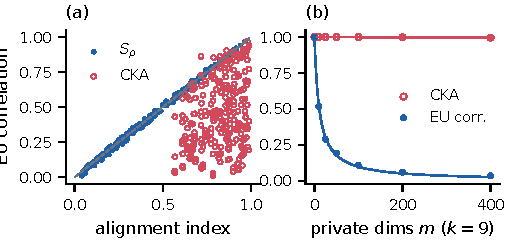
\includegraphics[width=\columnwidth]{figures/fig_theory.pdf}
\caption{\textbf{(a)} Empirical EU correlation versus $\Srho$ (filled) and CKA (open) over 60 synthetic pairs and four $\rho$. \textbf{(b)} The construction of \Cref{cor:neither} ($k=9$, $\lambda_s=10$, $\lambda_p=0.1$, $\rho=0.01$): CKA stays near one as private dimensions are added while EU correlation falls as $kw_s^2/(kw_s^2+mw_p^2)$; lines are the exact closed forms of \Cref{cor:neither}.}
\label{fig:theory}
\end{figure}

\subsection{Identical features, different heads (E2)}
\label{sec:e2}
\begin{table}[t]
\centering
\caption{E2: heads on \emph{identical} frozen features (all alignment metrics $=1$). Item-level Spearman agreement, mean (min--max) over five encoders; partial = controlling for both models' confidence and human entropy.}
\label{tab:e2}
\setlength{\tabcolsep}{3pt}
\resizebox{\columnwidth}{!}{%
\begin{tabular}{lccc}
\toprule
pair & EU width & EU partial & AU \\
\midrule
re-test floor & 1.00 (0.99--1.00) & 0.56 & 1.00 (1.00--1.00) \\
25\% vs 100\% data & 0.94 (0.90--0.96) & 0.36 & 0.94 (0.91--0.97) \\
10\% vs 100\% data & 0.90 (0.84--0.94) & 0.26 & 0.90 (0.85--0.94) \\
disjoint halves & 0.91 (0.88--0.94) & 0.36 & 0.92 (0.89--0.95) \\
wd $\div10$ & 0.98 (0.98--0.99) & 0.24 & 0.98 (0.97--0.99) \\
wd $\times10$ & 0.97 (0.97--0.98) & 0.49 & 0.97 (0.96--0.98) \\
\bottomrule
\end{tabular}}
\end{table}

Within each encoder the paired heads see literally the same features, so CKA and every other alignment index equals one.
Raw EU agreement is high for all pairs (\Cref{tab:e2}), but this is shared confidence: for softmax probes the bootstrap width has rank correlation \CorrWidthConfMin{} to \CorrWidthConfMax{} with the max-probability and at least \CorrWidthAUMin{} with AU on every encoder, whereas the closed-form $u(x)$, which ignores labels, correlates with it at only \CorrWidthBLRMin{} to \CorrWidthBLRMax{}.
We therefore read E2 through the partial agreement, controlling for both heads' confidence and human entropy.
It falls from a re-test value of \EtwoRetestPartial{} (two ensembles with identical configuration) to \EtwoHalvesPartial{} for disjoint halves of the training set and \EtwoFracTenPartialMean{} for 10\% versus 100\% of the data (\Cref{fig:e2} in the supplement).
Because the head objective averages the loss, the weight decay sets the same $\rho$ at every sample size, so this drop reflects the finite-sample data term (\Cref{sec:synthetic}) rather than the change of $\rho$ in \Cref{cor:same}; weight decay was not re-selected for subset heads.
Falsifier F-data ($>0.9$) is \EtwoFalsA{}, but in hindsight it could not have fired, since the re-test value itself is far below $0.9$ (\Cref{tab:prereg}).

\paragraph{Estimator noise and redraws (exploratory).}
The re-test partial agreement is limited by Monte Carlo noise: for DINOv2 it rises from \McurveWten{} at $M=10$ to \McurveWfifty{} at $M=50$ and \McurveWtwohundred{} at $M=200$ (\Cref{fig:rev}a).
We therefore repeated the identical-features analysis at $M=200$ for \MtwoEncs{} encoders, with three independent subset draws and the two weight-decay pairs, and divided each partial agreement by the geometric mean of the two heads' own re-test reliabilities (\Cref{tab:redraw}).
The reliability-corrected EU agreement is \MtFracWCorr{} for 10\% versus 100\% of the data and \MtHalfWCorr{} for disjoint halves; across encoders and draws the 95\% item-bootstrap intervals reach at most \MtFracWCorrHi{} and \MtHalfWCorrHi{}, so the disagreement is not estimator noise.
Two caveats bound the interpretation.
First, after the controls the residual holds only \ResidFracMin{}--\ResidFracMax{} of the rank variance of the bootstrap width: the finding concerns the fine structure of EU beyond confidence, not which inputs are most uncertain.
Second, this residual has no external validation as an epistemic quantity.
At the decision level, the overlap of the 10\% highest-uncertainty (acquisition) sets is \RdRetestWTop{} between re-test ensembles but \RdFracWTop{} between the 10\% and 100\% heads ($M=50$).
Replacing the plug-in human entropy by the Dirichlet-posterior estimator or by two independent split-half entropies changes the partial agreements by at most \SensMaxDiff{}, because confidence absorbs almost all shared variance.

Falsifier F-AU is \EtwoFalsB{}: AU agreement on identical features degrades about as much as EU agreement (raw drop \EtwoDropAU{} vs.\ \EtwoDropEU{}; corrected agreement at $M=200$: AU \MtFracAUCorr{} vs.\ EU \MtFracWCorr{}).
The pre-registered contrast that AU agreement is protected is not supported for softmax probes, consistent with the near-collinearity of their AU and EU summaries.
In an exploratory observation, AU's relation to the human target is stable: per encoder, Spearman between model AU and human entropy varies by at most \AUHumanRangeMax{} across the eight head configurations, at \AUHumanMin{}--\AUHumanMax{} overall (\AUHumanNormMin{}--\AUHumanNormMax{} of the attainable maximum $\sqrt{\CeilingCIFARh}=\SqrtCeiling$).



\begin{table}[t]
\centering
\caption{Heads on identical features at $M=200$ (exploratory): mean over 5 encoders (and 3 subset draws where applicable). Partial = controlling for both heads' confidence and human entropy; corrected = partial divided by the geometric mean of the two heads' re-test partial reliabilities, with the range of 95\% item-bootstrap intervals across encoders and draws; resid.\ = fraction of rank variance of EU width left after the controls.}
\label{tab:redraw}
\setlength{\tabcolsep}{2.5pt}
\resizebox{\columnwidth}{!}{%
\begin{tabular}{llcccc}
\toprule
pair & & raw & partial & corrected [95\% range] & resid. \\
\midrule
re-test & EU width & 1.00 & 0.79 & 1 & 0.3\% \\
 & AU & 1.00 & 0.94 & 1 & 0.2\% \\
wd $\div10$ & EU width & 0.99 & 0.35 & 0.42 [0.15, 0.87] & 0.3\% \\
 & AU & 0.99 & 0.29 & 0.31 [-0.05, 0.90] & 0.2\% \\
wd $\times10$ & EU width & 0.98 & 0.63 & 0.74 [0.53, 0.84] & 0.3\% \\
 & AU & 0.98 & 0.57 & 0.59 [0.23, 0.81] & 0.2\% \\
disjoint halves & EU width & 0.92 & 0.47 & 0.63 [0.44, 0.79] & 0.3\% \\
 & AU & 0.92 & 0.53 & 0.57 [0.42, 0.70] & 0.3\% \\
10\% vs 100\% & EU width & 0.90 & 0.34 & 0.43 [0.20, 0.58] & 0.3\% \\
 & AU & 0.91 & 0.45 & 0.48 [0.30, 0.65] & 0.2\% \\
\bottomrule
\end{tabular}}
\end{table}

\subsection{Transformations that preserve alignment (E2b)}
\label{sec:e2b}
\begin{table*}[t]
\centering
\caption{E2b (fixed weight decay): alignment of the transformed to the original features, Spearman rank agreement of EU with the untransformed head, and mean EU relative to it, for both encoders (width = bootstrap quantile width; Laplace = MI for the rank, logit variance for the ratio). The text summarises ranges over both encoders.}
\label{tab:e2b}
\setlength{\tabcolsep}{3pt}
\small
\begin{tabular}{lcccccccccccc}
\toprule
 & \multicolumn{6}{c}{DINOv2-B} & \multicolumn{6}{c}{CLIP-B/16} \\ \cmidrule(lr){2-7}\cmidrule(lr){8-13}
 & CKA & mKNN & \multicolumn{2}{c}{rank agr.} & \multicolumn{2}{c}{mean ratio} & CKA & mKNN & \multicolumn{2}{c}{rank agr.} & \multicolumn{2}{c}{mean ratio} \\
transform & & & width & Lapl. & width & Lapl. & & & width & Lapl. & width & Lapl. \\
\midrule
$c=$0.1 & 1.000 & 1.00 & 0.94 & 0.89 & 0.56 & 0.017 & 1.000 & 1.00 & 0.89 & 0.85 & 0.38 & 0.0301 \\
$c=$0.3 & 1.000 & 1.00 & 0.98 & 0.94 & 0.74 & 0.125 & 1.000 & 1.00 & 0.96 & 0.95 & 0.62 & 0.182 \\
$c=$1.0 & 1.000 & 1.00 & 1.00 & 1.00 & 1.00 & 1 & 1.000 & 1.00 & 1.00 & 1.00 & 1.00 & 1 \\
$c=$3.0 & 1.000 & 1.00 & 0.99 & 0.91 & 1.29 & 6.78 & 1.000 & 1.00 & 0.98 & 0.92 & 1.45 & 4.24 \\
$c=$10.0 & 1.000 & 1.00 & 0.97 & 0.85 & 1.52 & 61.7 & 1.000 & 1.00 & 0.95 & 0.72 & 1.84 & 39.3 \\
tail $s=$0.5 & 1.000 & 0.96 & 1.00 & 1.00 & 1.02 & 0.894 & 1.000 & 0.95 & 1.00 & 0.99 & 0.98 & 0.788 \\
tail $s=$2.0 & 0.998 & 0.89 & 1.00 & 0.99 & 1.07 & 1.27 & 0.999 & 0.86 & 0.99 & 0.98 & 1.13 & 1.47 \\
tail $s=$4.0 & 0.956 & 0.68 & 0.98 & 0.95 & 1.30 & 1.8 & 0.982 & 0.62 & 0.97 & 0.92 & 1.39 & 2.28 \\
\bottomrule
\end{tabular}
\end{table*}
Applying $\phi\mapsto cQ\phi$ leaves CKA and mutual $k$-NN at one for both encoders tested (DINOv2 and CLIP; \Cref{tab:e2b}).
\EtwobScaleText{}
The effect therefore operates through the prior, as \Cref{prop:scale} says; it vanishes when the weight decay is re-tuned.
The point is not that practitioners will meet this failure after tuning, but that CKA cannot tell whether two heads' priors are matched to their feature scales.
Tail reshaping (scaling the directions outside the top 95\% of variance by $s\in\{0.5,2,4\}$) keeps CKA at or above \EtwobTailCKAMin{} while the mean Laplace logit variance changes by up to a factor \EtwobTailLapMax{} and the mean bootstrap width by up to \EtwobTailWidthMax{} (ranges over both encoders); mutual $k$-NN, which is sensitive to the tail, drops to \EtwobTailMKNNMin{}.
The closed-form EU barely moves (mean ratio within \EtwobTailBLRdev{} of one): at the selected weight decay the heads are in the small-$\rho$ regime, where $u(x)$ approaches the leverage, which is invariant to every invertible linear map.
The softmax estimators move because their effective prior strength is set by the curvature of the likelihood, not by the weight decay alone.
\Cref{lem:boot} predicts that bootstrap EU moves less than Laplace EU under tail reshaping; this held in \EtwobBootLessLaplace{} settings (3 values of $s$ $\times$ 2 encoders, comparing rank changes). The lemma is derived for residual resampling, so this is a heuristic extrapolation to Poisson-resampled softmax heads.

\subsection{Across encoders: which index tracks EU agreement?}
\label{sec:srho}
\begin{table*}[t]
\centering
\caption{Across 30 encoder pairs (5 encoders $\times$ 3 depths): Spearman correlation between each alignment index and item-level agreement, on all pairs and (in parentheses) its range over the five leave-one-encoder-out subsets of 18 pairs. With five encoders no valid sampling interval is available; the ranges are descriptive. Bottom rows: differences, with the number of subsets in which they are positive.}
\label{tab:srho}
\resizebox{\textwidth}{!}{%
\begin{tabular}{lccc}
\toprule
index & width (partial) & closed form & AU \\
\midrule
CKA & 0.64 (0.62--0.67) & 0.76 (0.62--0.89) & 0.68 (0.54--0.84) \\
mutual $k$-NN & 0.72 (0.69--0.89) & 0.90 (0.85--0.95) & 0.86 (0.75--0.91) \\
linear predictivity & 0.83 (0.79--0.90) & 0.56 (0.35--0.74) & 0.53 (0.39--0.78) \\
$S_{\rho\to0}$ & 0.83 (0.77--0.90) & 0.93 (0.87--0.96) & 0.93 (0.89--0.92) \\
$S_\rho$ (head's $\rho$) & 0.83 (0.76--0.90) & 0.92 (0.84--0.95) & 0.92 (0.87--0.92) \\
\midrule
$S_\rho-$CKA & +0.19 (+0.09 to +0.26; 5/5 $>0$) & +0.16 (-0.02 to +0.30; 4/5 $>0$) & +0.24 (+0.08 to +0.33; 5/5 $>0$) \\
$S_\rho-$mutual $k$-NN & +0.11 (-0.04 to +0.17; 4/5 $>0$) & +0.03 (-0.08 to +0.09; 3/5 $>0$) & +0.07 (+0.00 to +0.12; 4/5 $>0$) \\
$S_\rho-$linear pred. & -0.00 (-0.08 to +0.05; 1/5 $>0$) & +0.37 (+0.11 to +0.52; 5/5 $>0$) & +0.40 (+0.13 to +0.53; 5/5 $>0$) \\
\bottomrule
\end{tabular}}
\end{table*}
For all 10 encoder pairs at three matched relative depths (30 pairs) we compute CKA, mutual $k$-NN ($k=10$), symmetric linear predictivity, $\Srho$ at the two heads' own $\rho$ and its $\rho\to0$ limit, on training $\cup$ test inputs, together with item-level EU agreement (\Cref{tab:srho}; scatter plots in \Cref{fig:real} of the supplement).
For partial bootstrap EU agreement, $\Srho$, $S_{\rho\to0}$ and linear predictivity all reach \SrhoVsEUwidthPartial{}, mutual $k$-NN \MKNNVsEUwidthPartial{} and CKA \CKAVsEUwidthPartial{}.
This ordering is what \Cref{prop:limits} predicts for weakly regularised heads, but the evidence is limited: pairs share encoders, and with five encoders no resampling scheme gives a valid interval. We therefore report how the comparison changes when each encoder is left out (\Cref{tab:srho}): $\Srho-\mathrm{CKA}$ stays positive in \LOEOdiffCKApos{}/5 subsets (\LOEOdiffCKAmin{} to \LOEOdiffCKAmax{}) for partial agreement and in \LOEOdiffCKAblrPos{}/5 for closed-form agreement, whereas the differences from linear predictivity (\LOEOdiffLinMin{} to \LOEOdiffLinMax{}) and mutual $k$-NN (\LOEOdiffMknnMin{} to \LOEOdiffMknnMax{}) change sign.
$\Srho$ is also indistinguishable from its own $\rho\to0$ limit, so at the selected weight decays we cannot attribute any advantage to the head's prior strength.
Falsifier S (``no better than CKA'') is \SrhoFals{} on the point estimate; we classify the prediction as inconclusive.
The three indices that do well are all tail-sensitive, and two of them (CCA-type, mutual $k$-NN) are as scale-blind as CKA: the comparison isolates spectral weighting, not scale.
CKA is not uninformative, and for raw agreement linear predictivity (\LinVsEUwidth{}) is weaker still; the highest-CKA pair at the final depth (CKA \EfourCKA{}) reaches a partial EU agreement of only \HighCKAPartial{}.
$\Srho$, its $\rho\to0$ limit and mutual $k$-NN predict AU agreement about as well as EU agreement ($\Srho$: \SrhoVsAU{}; linear predictivity is the exception), so they index shared head behaviour rather than EU specifically.
On real features \Cref{thm:identity} holds only ordinally: $\Srho$ ranks the \emph{Pearson} agreement of the closed form, the quantity in \Cref{thm:identity} (Table~\ref{tab:srho} uses Spearman), at \RealThmRank{} (CKA: \RealThmRankCKA{}) but its level is off by \RealThmMAE{}. The offset is due to non-Gaussianity: replacing each pair's features by Gaussian draws with the same joint covariance reduces the mean absolute error between $\Srho$ and the closed-form Pearson agreement from \GaussMAEreal{} to \GaussMAEgauss{}, so the identity is exact up to higher cumulants.

\paragraph{Does the head's $\rho$ matter? (exploratory).}
At the selected weight decays all heads have $\deff(\rho)/d>0.98$, so $\Srho\approx S_{\rho\to0}$.
We therefore refit all 15 encoder--depth heads ($M=20$) at a common weight decay $\rho\in\{10^{-3},10^{-2},10^{-1},1\}$, which lowers $\deff(\rho)/d$ to \SweepDeffMin{}--\SweepDeffMax{} at $\rho=1$ (\Cref{fig:rev}b).
As predicted, the advantage of evaluating the index at the matched $\rho$ grows with $\rho$: for closed-form EU agreement $\Srho-S_{\rho\to0}$ moves from \SweepDiffSmallBLR{} at $\rho=10^{-3}$ to \SweepDiffBLR{} at $\rho=1$ (\SweepBLRsrho{} vs.\ \SweepBLRszero{}; CKA \SweepBLRcka{}), and for partial bootstrap agreement to \SweepDiffW{} (\SweepWsrho{} vs.\ \SweepWszero{}; CKA \SweepWcka{}).
At $\rho=1$ the difference is positive in \SweepLOEOposBLR{}/5 (closed form) and \SweepLOEOposW{}/5 (partial bootstrap) leave-one-encoder-out subsets, but strongly regularised heads underfit for some encoders (accuracy \SweepAccMin{}--\SweepAccMax{}), and the weight decay of a softmax head is not its effective prior strength (\RhoEffText{}), so this is a trend, not an established effect.
Computing $\Srho$ on training inputs only instead of training $\cup$ test changes its correlation with EU agreement by at most \SweepTrainOnlyMaxDiff{}.
Evaluating $\Srho$ at the curvature-calibrated $\rho_{\mathrm{eff}}$ of each softmax head (median \RhoEffMed{}, range \RhoEffMin{}--\RhoEffMax{}) does not help either: it correlates with partial bootstrap agreement at \SrhoEffVsEUwidthPartial{}, below its $\rho\to0$ limit (\SzeroVsEUwidthPartial{}), so for softmax probes we cannot confirm the matched-prior prediction.
Between different encoders, the top-10\% acquisition sets overlap by only \CrossTopTen{} on average.

\begin{figure}[t]
\centering
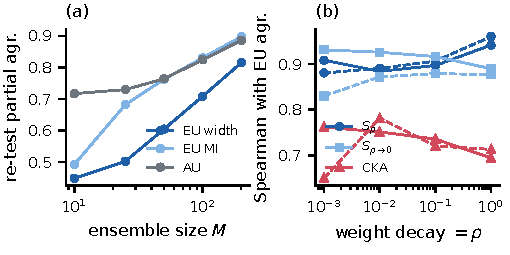
\includegraphics[width=\columnwidth]{figures/fig_rev.pdf}
\caption{Exploratory analyses. \textbf{(a)} Re-test partial agreement of two independent ensembles versus ensemble size $M$ (DINOv2, final layer; seeds independent of \Cref{tab:e2}, hence 0.60 vs.\ 0.61 at $M=50$): the noise floor in \Cref{tab:e2} is a Monte Carlo limit. \textbf{(b)} Weight-decay sweep over 30 encoder pairs: Spearman correlation of $\Srho$ at the matched $\rho$, its $\rho\to0$ limit and CKA with closed-form (solid) and partial bootstrap (dashed) EU agreement.}
\label{fig:rev}
\end{figure}

\paragraph{Label-free prediction.}
Across encoders and depths, $\deff(\rho)$ from unlabelled training features rank-correlates with mean closed-form EU at \DeffVsBLR{}, as \Cref{lem:deff} predicts, but not with the mean bootstrap width of softmax heads (\DeffVsWidth{}), whose magnitude follows accuracy; this pre-registered prediction failed for softmax heads.

\paragraph{Swap design (E4).}
In a $2\times2\times2$ design on the highest-CKA pair (DINOv2-B vs.\ supervised ViT-B/16, CKA \EfourCKA{}; encoder $\times$ weight decay $\{w,10w\}$ $\times$ disjoint training half), the encoder accounts for \EfourRep{} of the Shapley decomposition of raw EU disagreement, the training half for \EfourData{} and the weight decay for essentially none (\EfourHead{}).
This triggers the pre-registered E4 falsifier ($>80\%$): among the encoders we could test, alignment never reached a regime where head and data terms dominate.
In an exploratory variant using partial disagreement, the shares are \EfourPRep{}, \EfourPData{} and \EfourPHead{} for encoder, data and weight decay (re-test disagreement \EfourPFloor{}).



\section{DISCUSSION}
\label{sec:disc}

\paragraph{What the results say.}
That a representation-only index cannot determine EU follows from \Cref{eq:blr}; our contribution is to say which information an index needs and why CKA lacks it.
\Cref{thm:identity} identifies the relevant summary for linear-Gaussian heads, spectral overlap above the head's prior strength weighted by $w_i(\rho)^2$, and is compatible with two observations: tail-sensitive indices (CCA-type, mutual $k$-NN, linear predictivity) tracked EU agreement better than CKA for weakly regularised heads, and the matched-$\rho$ index gained ground as regularisation increased.
Because every well-performing index except $\Srho$ is scale-invariant, the cross-encoder data support the spectral-weighting mechanism, not the scale mechanism; the latter is supported only by the controlled transformations of \Cref{sec:e2b}.
With five encoders neither cross-encoder difference is statistically established.
Two further observations are diagnostic rather than practical. CKA's invariance to scale hides a prior--scale mismatch that moves EU by orders of magnitude (pre-registered, E2b), although the mismatch disappears once the weight decay is tuned, as \Cref{prop:scale} implies. And in exploratory redraws, identical features leave the confidence-residual EU ranking dependent on the training data (\Cref{sec:e2}); this residual is a small part of the total rank variance, so the observation concerns fine structure rather than which inputs are most uncertain.
Between different encoders, however, the representation is the dominant source of EU disagreement (E4), so our results do not say that the encoder is irrelevant; they say that CKA does not tell us how EU will agree.
For softmax probes, EU and AU summaries are nearly collinear with confidence, so the empirical part of this paper cannot separate EU-specific from general head agreement; the EU-specific mechanisms are established by the theory and the closed form.

\paragraph{Recommendations.}
(i) \emph{Supported:} do not use CKA to transfer or validate EU. \emph{Conjecture, not established here:} tail-sensitive indices are better proxies; among them, only $\Srho$ evaluated at the head's prior strength on the head's own feature scaling also reflects a prior--scale mismatch ($\Srho(cQ\phi)=S_{\rho/c^2}(\phi)$). Whitened indices can be unstable when the dimension is large relative to the sample, which $\Srho$ regularises. We found no advantage of $\Srho$ over linear predictivity or mutual $k$-NN at the weight decays practitioners select.
(ii) Report the weight decay together with the feature normalisation used (here a single scalar on centred features), since the pair determines the effective prior; for Laplace heads, report the prior precision relative to the trace of the feature covariance.
(iii) Report confidence-controlled (partial) agreement with re-test reliabilities, since raw EU agreement of softmax probes mostly reflects shared confidence and the partial measure is noisy at common ensemble sizes.

\paragraph{Limitations.}
The theory is exact for Gaussian features and linear-Gaussian heads; on real features only its ordinal predictions held.
Softmax heads enter through bootstrap and Laplace approximations; the bootstrap lemma is for residual resampling with fixed design, and our Laplace drops cross-class curvature.
Five encoders give 30 dependent pairs, which limits every cross-encoder conclusion, and the encoder set has no model-scale axis, so we cannot speak to the scale-dependent convergence trend of \citet{huh2024platonic}.
For softmax probes our empirical EU summaries are confounded with confidence; an EU target that separates from confidence (e.g.\ out-of-distribution inputs or held-out classes) and closed-form or Gaussian-process heads as the primary empirical object are the natural next steps.
We study frozen encoders and linear probes on one dataset with human labels (CIFAR-10H) at low native resolution and only in-distribution; out-of-distribution inputs, where shared blind spots matter most, fine-tuned models, other modalities and the DCIC datasets are not covered, and we do not evaluate downstream active-learning performance.
The positive control replaces the planned DCIC synthetic dataset with a known softmax teacher on each encoder's features.
Additional analyses not in the pre-registration (\Cref{fig:rev}, \Cref{tab:redraw}, leave-one-encoder-out ranges) are exploratory.
Planned analyses that were not run (class/residual decomposition, AU-versus-function agreement, robustness to $k$, pooling and probe class) are not claimed.

\subsection*{AI use statement}
% TODO(authors): after your own line-by-line proof check, add "and line by line by the authors" after "random instances". Do not add it before.
We used generative AI tools (a large language model coding and writing assistant) for implementation of the experiment code from the authors' design scaffold, numerical verification of theoretical claims, drafting of proofs, drafting and editing of the manuscript text, generation of figures and tables, assembly of the bibliography, and a simulated multi-reviewer critique whose findings informed this revision. The research question, pre-registered predictions and falsifiers, and experimental design were specified by the authors before AI assistance. All AI-generated code was checked against independent reference implementations by unit tests (17 tests, including 9 theory checks), every proof was checked numerically on random instances, and every number in the paper is generated by script from logged results. We take responsibility for the final content of this work, including text, claims, and artifacts produced with the aid of generative AI.

\bibliography{refs}

\clearpage
\section*{Checklist}

\begin{enumerate}

  \item For all models and algorithms presented, check if you include:
  \begin{enumerate}
    \item A clear description of the mathematical setting, assumptions, algorithm, and/or model. [Yes] \Cref{sec:setup,sec:theory}.
    \item An analysis of the properties and complexity (time, space, sample size) of any algorithm. [Yes] $\Srho$ needs only $d\times d$ matrices, $O(nd^2+d^3)$ (\Cref{sec:theory}); compute in \Cref{app:details}.
    \item (Optional) Anonymized source code, with specification of all dependencies, including external libraries. [Yes] Supplementary code with \texttt{requirements.txt}.
  \end{enumerate}

  \item For any theoretical claim, check if you include:
  \begin{enumerate}
    \item Statements of the full set of assumptions of all theoretical results. [Yes] Each statement lists its assumptions (Gaussian features, linear-Gaussian heads, fixed design where relevant).
    \item Complete proofs of all theoretical results. [Yes] \Cref{app:proofs}.
    \item Clear explanations of any assumptions. [Yes] \Cref{sec:theory,sec:disc}.
  \end{enumerate}

  \item For all figures and tables that present empirical results, check if you include:
  \begin{enumerate}
    \item The code, data, and instructions needed to reproduce the main experimental results (either in the supplemental material or as a URL). [Yes] Supplementary code; public datasets and weights.
    \item All the training details (e.g., data splits, hyperparameters, how they were chosen). [Yes] \Cref{sec:exp,app:details}.
    \item A clear definition of the specific measure or statistics and error bars (e.g., with respect to the random seed after running experiments multiple times). [Yes] \Cref{app:details}; re-test floors quantify bootstrap seed variability.
    \item A description of the computing infrastructure used. (e.g., type of GPUs, internal cluster, or cloud provider). [Yes] \Cref{app:details}.
  \end{enumerate}

  \item If you are using existing assets (e.g., code, data, models) or curating/releasing new assets, check if you include:
  \begin{enumerate}
    \item Citations of the creator If your work uses existing assets. [Yes]
    \item The license information of the assets, if applicable. [Yes] \Cref{app:details}.
    \item New assets either in the supplemental material or as a URL, if applicable. [Yes] Code only.
    \item Information about consent from data providers/curators. [Not Applicable]
    \item Discussion of sensible content if applicable, e.g., personally identifiable information or offensive content. [Not Applicable]
  \end{enumerate}

  \item If you used crowdsourcing or conducted research with human subjects, check if you include:
  \begin{enumerate}
    \item The full text of instructions given to participants and screenshots. [Not Applicable] We use the public CIFAR-10H labels.
    \item Descriptions of potential participant risks, with links to Institutional Review Board (IRB) approvals if applicable. [Not Applicable]
    \item The estimated hourly wage paid to participants and the total amount spent on participant compensation. [Not Applicable]
  \end{enumerate}

\end{enumerate}


\clearpage
\appendix
\thispagestyle{empty}
\onecolumn
\aistatstitle{When Do Aligned Representations Agree on What They Do Not Know? \\ Supplementary Materials}
\section{PROOFS}
\label{app:proofs}

Throughout, $w_i(\rho)=\lambda_i/(\lambda_i+\rho)$, and $M$ matrices are symmetric.

\paragraph{Proof of \Cref{thm:identity}.}
Write $a=\phi_A(x)$, $b=\phi_B(x)$, $P=M_A$, $Q=M_B$. For a zero-mean Gaussian vector, Isserlis' theorem \citep{isserlis1918} gives
$\E[a_ia_jb_kb_l]=(\Sigma_A)_{ij}(\Sigma_B)_{kl}+(\Sigma_{AB})_{ik}(\Sigma_{AB})_{jl}+(\Sigma_{AB})_{il}(\Sigma_{AB})_{jk}$.
Contracting with $P_{ij}Q_{kl}$ and using the symmetry of $P,Q$,
\[
\E[a^\top Pa\; b^\top Qb]=\tr(P\Sigma_A)\tr(Q\Sigma_B)+2\tr(P\Sigma_{AB}Q\Sigma_{BA}).
\]
Since $\E[a^\top Pa]=\tr(P\Sigma_A)$, $\mathrm{Cov}(a^\top Pa,b^\top Qb)=2\tr(P\Sigma_{AB}Q\Sigma_{BA})$. Setting $b=a$, $Q=P$ gives $\mathrm{Var}(a^\top Pa)=2\tr((P\Sigma_A)^2)$, and likewise for $b$. Dividing gives $S(M_A,M_B)$. For $u_A,u_B$ take $M_A=(\Sigma_A+\rho_AI)^{-1}$, $M_B=(\Sigma_B+\rho_BI)^{-1}$. \hfill$\square$

\paragraph{Proof of \Cref{prop:limits}.}
(i) As $\rho\to\infty$, $\rho M_A\to I$ and $\rho M_B\to I$. Multiplying numerator and both factors of the denominator by $\rho^2$, the numerator tends to $\tr(\Sigma_{AB}\Sigma_{BA})=\|\Sigma_{AB}\|_F^2$ and the denominator to $\sqrt{\tr(\Sigma_A^2)\tr(\Sigma_B^2)}=\|\Sigma_A\|_F\|\Sigma_B\|_F$.
(ii) As $\rho\to0$, $M_A\to\Sigma_A^{-1}$; the numerator tends to $\tr(\Sigma_A^{-1}\Sigma_{AB}\Sigma_B^{-1}\Sigma_{BA})=\|\Sigma_A^{-1/2}\Sigma_{AB}\Sigma_B^{-1/2}\|_F^2=\sum_jr_j^2$, and $\tr((\Sigma_A^{-1}\Sigma_A)^2)=d_A$. The limit is therefore $\sum_jr_j^2/\sqrt{d_Ad_B}$, which equals the mean squared canonical correlation only when $d_A=d_B$. \hfill$\square$

\paragraph{Proof of \Cref{cor:neither}.}
$\Sigma_{AB}=\mathrm{diag}(\lambda_sI_k,0)$ and $M_A=\mathrm{diag}((\lambda_s+\rho)^{-1}I_k,(\lambda_p+\rho)^{-1}I_m)$, so the numerator of $\Srho$ is $kw_s^2$ and $\tr((M_A\Sigma_A)^2)=kw_s^2+mw_p^2$; CKA follows the same way with $\lambda$ in place of $w$.
\emph{High CKA, low agreement:} take $\rho\le\lambda_p$ (so $w_p\ge\frac12$, $w_s\le1$) and $m\ge4k/\epsilon$; then $\corr\le k/(k+m/4)\le\epsilon$. Then take $\lambda_p/\lambda_s\le\sqrt{\epsilon k/m}$, so $\cka=1/(1+(m/k)(\lambda_p/\lambda_s)^2)\ge1/(1+\epsilon)\ge1-\epsilon$.
\emph{Low CKA, high agreement:} take $\rho\le\lambda_s$ (so $w_s\ge\frac12$) and $k\ge4m/\epsilon$; then $\corr=1/(1+mw_p^2/(kw_s^2))\ge1-4m/k\ge1-\epsilon$. Then take $\lambda_p/\lambda_s\ge\sqrt{k/(m\epsilon)}$, so $\cka\le k\lambda_s^2/(m\lambda_p^2)\le\epsilon$. \hfill$\square$

\paragraph{Proof of \Cref{prop:scale}.}
CKA and cosine similarities are invariant to $\phi\mapsto cQ\phi$. For the variance,
$v(cQ\Phi,cQx;\lambda)=\sigma^2c^2x^\top Q^\top(c^2Q\Phi^\top\Phi Q^\top+\lambda I)^{-1}Qx=\sigma^2x^\top(\Phi^\top\Phi+(\lambda/c^2)I)^{-1}x$.
So the transformed head is the original head with prior strength $\rho/c^2$. Apply \Cref{thm:identity} to the same features with $M_A=(\Sigma+\rho c^{-2}I)^{-1}$, $M_B=(\Sigma+\rho I)^{-1}$, $\Sigma_{AB}=\Sigma$: the numerator is $\sum_iw_i(\rho/c^2)w_i(\rho)$ and the denominators are $\sum_iw_i(\cdot)^2$. By Cauchy--Schwarz the ratio equals one iff $w_i(\rho)/w_i(\rho/c^2)=(\lambda_i+\rho/c^2)/(\lambda_i+\rho)$ is constant over the support, i.e.\ iff the nonzero $\lambda_i$ are equal (for $c\ne1$). \hfill$\square$

\paragraph{Proof of \Cref{prop:tail}.}
With $T_s=U\,\mathrm{diag}(s_i)U^\top$ ($s_i=s$ on $\mathcal T$, $1$ otherwise), $\E[\phi(T_s\phi)^\top]=U\Lambda\,\mathrm{diag}(s_i)U^\top$ and $\mathrm{Cov}(T_s\phi)=U\Lambda\,\mathrm{diag}(s_i^2)U^\top$. Hence
$\cka=\sum\lambda_i^2s_i^2/\sqrt{\sum\lambda_i^2\sum\lambda_i^2s_i^4}=(1+s^2\eta)/\sqrt{(1+\eta)(1+s^4\eta)}$.
Moreover $1-\cka^2=\eta(s^2-1)^2/((1+\eta)(1+s^4\eta))\le\eta(s^2-1)^2$, and $\cka\ge\cka^2$ since $\cka\le1$. The transformed eigenvalues are $s^2\lambda_i$ on $\mathcal T$, and $s^2\lambda_i/(s^2\lambda_i+\rho)=w_i(\rho/s^2)$. \hfill$\square$

\paragraph{Proof of \Cref{lem:deff}.}
$\sum_iv(x_i)=\sigma^2\tr(\Phi(\Phi^\top\Phi+\lambda I)^{-1}\Phi^\top)=\sigma^2\sum_ig_i/(g_i+\lambda)$ with $g_i=n\hat\lambda_i$ the eigenvalues of $\Phi^\top\Phi$; divide by $n$ and use $\lambda/n=\rho$. \hfill$\square$

\paragraph{Proof of \Cref{cor:same}.} \Cref{thm:identity} with $\Sigma_A=\Sigma_B=\Sigma_{AB}=\Sigma$, $M_j=(\Sigma+\rho_jI)^{-1}$. \hfill$\square$

\paragraph{Proof of \Cref{lem:boot}.}
With $y=\Phi w+\varepsilon$, $\mathrm{Cov}(\varepsilon)=\sigma^2I$ and $\hat w=A^{-1}\Phi^\top y$, $\mathrm{Cov}_\varepsilon(\hat w)=\sigma^2A^{-1}\Phi^\top\Phi A^{-1}=\sigma^2A^{-1}GA^{-1}$. In the eigenbasis of $G$ this is $\sigma^2g_i/(g_i+\lambda)^2$, against the posterior $\sigma^2/(g_i+\lambda)$. Residual resampling estimates this noise covariance as $n\to\infty$. The EU score is $\phi^\top\mathrm{Cov}(\hat w)\phi=\frac{\sigma^2}{n}\phi^\top(\hat\Sigma+\rho)^{-1}\hat\Sigma(\hat\Sigma+\rho)^{-1}\phi$, so in \Cref{thm:identity} $M\Sigma$ has eigenvalues $w_i^2$ and the direction weights are $w_i^4$. \hfill$\square$

\paragraph{Proof of \Cref{prop:resolvent}.}
$G$ and $(G+s^2I)^{-1}$ commute, so $\mathrm P(G)=G(G+s^2I)^{-1}[(G+s^2I)-G]=s^2(I-s^2(G+s^2I)^{-1})$. Hence $\mathrm P(K)-\mathrm P(L)=s^4[(L+s^2I)^{-1}-(K+s^2I)^{-1}]=s^4(K+s^2I)^{-1}(K-L)(L+s^2I)^{-1}$, and $\|(G+s^2I)^{-1}\|_{\mathrm{op}}\le s^{-2}$ for $G\succeq0$. \hfill$\square$

\paragraph{The bound fails for unobserved points.}
For $Z=\mathcal T\cup\mathcal E$ with only $\mathcal T$ observed, $\mathrm P(G)=G-G_{Z\mathcal T}(G_{\mathcal T\mathcal T}+s^2I)^{-1}G_{\mathcal TZ}$. In 3000 random trials (feature dimension 1--11, $|\mathcal T|\in[3,30)$, $|\mathcal E|\in[1,20)$, $s^2\in[10^{-2},10]$) the ratio $\|\mathrm P(K)-\mathrm P(L)\|_{\mathrm{op}}/\|K-L\|_{\mathrm{op}}$ reached \ResolventWorst{}, so no constant-one bound holds there.

\section{EXPERIMENTAL DETAILS}
\label{app:details}

\paragraph{Pre-registration.} The \texttt{PREREG} dictionary (claims, falsifiers, gate) was frozen before any real-data computation; its SHA-256 is \texttt{\PreregHashFull} (file \texttt{PREREG\_FROZEN.txt} in the supplementary code, frozen 2026-10-02 before any real-data computation; no external registry was used, so the hash certifies content, not time). The frozen falsifiers for E2-b (``AU degrades as much as EU'') and S (``no better than CKA'') carried no numeric threshold; the operational rules in \Cref{tab:prereg} were fixed by us when computing them and are therefore post hoc. Analyses not in the pre-registration (the $\Srho$ evaluation at $\rho\to0$, the $\deff$-versus-participation-ratio contrast, the exploratory E4 variant, and all post-review analyses in \Cref{app:revision}) are exploratory.

\paragraph{Features.} Taps at relative depths $0.5,0.75,1$ of the flattened block list; mean over patch tokens excluding prefix tokens (ViTs) or spatial mean (ConvNeXt) of the raw block output; fp16 cache; bicubic upsampling $32\to224$ with each encoder's own normalisation. DINOv2 uses \texttt{img\_size=224} with interpolated position embeddings.

\paragraph{Heads.} Softmax regression, objective $\sum_iw_i\,\mathrm{CE}_i/\sum_iw_i+\frac{\mathrm{wd}}2\|W\|^2$, full-batch L-BFGS (strong Wolfe, $\le200$ iterations), all $M$ members trained in one tensor; agreement with scikit-learn's optimum to $5\times10^{-4}$ in probability. Weight decay grid $\{10^{-5},\dots,10^{-1}\}$, chosen by validation NLL on a fixed 10k split of the training set with hard labels. Poisson(1) bootstrap weights. EU summaries: summed $5$--$95\%$ quantile width over classes and mutual information; AU: mean member entropy. Laplace: class-block-diagonal GGN at the MAP of member 0 with prior precision $n\cdot\mathrm{wd}$, 100 Monte Carlo logit samples. Closed-form EU: $u(x)=\phi^\top(\hat\Sigma+\rho I)^{-1}\phi$ with $\rho=\mathrm{wd}$.

\paragraph{Ensemble size.} \MChoice

\paragraph{Statistics.} Item-level Spearman; partial Spearman on ranks residualised on both models' confidence (max mean probability) and human plug-in entropy; stratified Spearman within human-entropy deciles. CIFAR-10H ceiling: split votes into halves without replacement (multivariate hypergeometric), Spearman between half entropies, Spearman--Brown corrected, 50 repetitions.

\paragraph{Compute.} One Apple M2 Pro laptop (16\,GB), PyTorch MPS for feature extraction (68--113 images/s) and CPU float32/float64 for heads and linear algebra.

\paragraph{Licences.} CIFAR-10H: CC BY-NC-SA 4.0. Model weights via \texttt{timm} and \texttt{open\_clip} under their respective licences.

\section{POST-REVIEW ANALYSES}
\label{app:revision}
All analyses in this section were added after an internal round of review and are exploratory.
\paragraph{Leave-one-encoder-out sensitivity.} The 30 encoder pairs share encoders, so they are not independent, and with five encoders a cluster bootstrap is degenerate (few distinct resamples, many with fewer than three pairs). We therefore recompute every correlation on the five subsets that leave out one encoder (18 pairs each) and report the range and the number of subsets in which a difference is positive. These ranges describe sensitivity; they are not confidence intervals. An earlier draft reported percentile cluster-bootstrap intervals, which we withdrew for this reason.
\paragraph{Reliability and redraws.} For each encoder (final depth, selected weight decay, $M=50$) we draw three independent 10\% subsets and three independent splits into halves; every head is fitted twice with different Poisson weights. A pair's corrected agreement is its partial agreement divided by $\sqrt{r_{xx}r_{yy}}$, where $r_{xx}$ is the partial agreement between the two replicates of head $x$. The re-test ensembles use seeds 0 and 1 of the full-data head. In the E2b re-tuning, the selected weight decays lie on the boundaries of the searched grid for $c=0.1$ and $c=10$, so the re-tuned values are bounds rather than interior optima.
\paragraph{Weight-decay sweep.} All 15 encoder--depth heads are refitted with $M=20$ at a common weight decay $\rho\in\{10^{-3},10^{-2},10^{-1},1\}$ (no validation selection), and agreement and indices are recomputed for the 30 pairs. Training-only $\Srho$ uses the same 10k training subset without test inputs.

\section{ADDITIONAL RESULTS}
\label{app:results}
\begin{figure}[h]
\centering
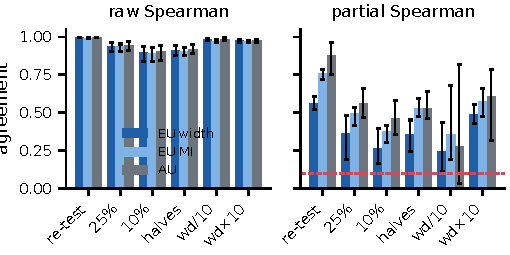
\includegraphics[width=0.6\textwidth]{figures/fig_e2.pdf}
\caption{E2: agreement between heads on identical features, mean over five encoders (bars: min--max). Right: partial Spearman controlling for both heads' confidence and human entropy; the dashed line is the mean partial EU agreement between \emph{different} encoders at the final depth.}
\label{fig:e2}
\end{figure}
\begin{figure}[h]
\centering
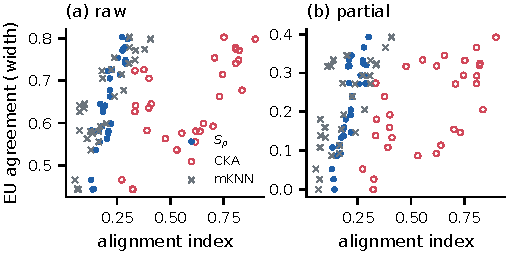
\includegraphics[width=0.6\textwidth]{figures/fig_real.pdf}
\caption{Across 30 encoder pairs (5 encoders, 3 depths): item-level bootstrap EU agreement, raw \textbf{(a)} and partial \textbf{(b)}, against $\Srho$ at the heads' $\rho$ (filled), CKA (open) and mutual $k$-NN (crosses).}
\label{fig:real}
\end{figure}

\begin{table}[h]
\centering
\caption{E2 per encoder: Spearman (partial) agreement for EU width, mutual information and AU, and model AU versus human entropy (fraction of ceiling).}
\small
\begin{tabular}{llccc}
\toprule
encoder & pair & EU width & EU MI & AU \\
\midrule
DINOv2-B & re-test floor & 1.00 (0.61) & 0.99 (0.78) & 1.00 \\
DINOv2-B & 25\% vs 100\% data & 0.96 (0.48) & 0.95 (0.54) & 0.97 \\
DINOv2-B & 10\% vs 100\% data & 0.94 (0.40) & 0.93 (0.42) & 0.94 \\
DINOv2-B & disjoint halves & 0.94 (0.45) & 0.93 (0.55) & 0.95 \\
DINOv2-B & wd $\div10$ & 0.99 (0.28) & 0.96 (0.19) & 0.99 \\
DINOv2-B & wd $\times10$ & 0.98 (0.55) & 0.98 (0.53) & 0.98 \\
DINOv2-B & AU vs human & \multicolumn{3}{c}{0.36 (0.43 of $\sqrt{\text{ceiling}}$); test acc. 0.98} \\ \midrule
CLIP-B/16 & re-test floor & 1.00 (0.52) & 0.99 (0.73) & 1.00 \\
CLIP-B/16 & 25\% vs 100\% data & 0.95 (0.33) & 0.94 (0.50) & 0.95 \\
CLIP-B/16 & 10\% vs 100\% data & 0.90 (0.21) & 0.89 (0.39) & 0.90 \\
CLIP-B/16 & disjoint halves & 0.91 (0.30) & 0.91 (0.52) & 0.92 \\
CLIP-B/16 & wd $\div10$ & 0.98 (0.11) & 0.97 (0.35) & 0.97 \\
CLIP-B/16 & wd $\times10$ & 0.97 (0.45) & 0.96 (0.58) & 0.96 \\
CLIP-B/16 & AU vs human & \multicolumn{3}{c}{0.43 (0.51 of $\sqrt{\text{ceiling}}$); test acc. 0.95} \\ \midrule
ViT-B/16 sup. & re-test floor & 1.00 (0.55) & 0.99 (0.72) & 1.00 \\
ViT-B/16 sup. & 25\% vs 100\% data & 0.95 (0.43) & 0.95 (0.49) & 0.96 \\
ViT-B/16 sup. & 10\% vs 100\% data & 0.93 (0.25) & 0.92 (0.30) & 0.93 \\
ViT-B/16 sup. & disjoint halves & 0.94 (0.39) & 0.93 (0.48) & 0.95 \\
ViT-B/16 sup. & wd $\div10$ & 0.99 (0.28) & 0.97 (0.21) & 0.99 \\
ViT-B/16 sup. & wd $\times10$ & 0.98 (0.43) & 0.97 (0.48) & 0.98 \\
ViT-B/16 sup. & AU vs human & \multicolumn{3}{c}{0.35 (0.42 of $\sqrt{\text{ceiling}}$); test acc. 0.98} \\ \midrule
ConvNeXt-S & re-test floor & 1.00 (0.55) & 0.99 (0.78) & 1.00 \\
ConvNeXt-S & 25\% vs 100\% data & 0.93 (0.39) & 0.93 (0.54) & 0.94 \\
ConvNeXt-S & 10\% vs 100\% data & 0.88 (0.28) & 0.88 (0.41) & 0.89 \\
ConvNeXt-S & disjoint halves & 0.88 (0.40) & 0.88 (0.59) & 0.89 \\
ConvNeXt-S & wd $\div10$ & 0.98 (0.12) & 0.97 (0.35) & 0.98 \\
ConvNeXt-S & wd $\times10$ & 0.97 (0.50) & 0.97 (0.63) & 0.97 \\
ConvNeXt-S & AU vs human & \multicolumn{3}{c}{0.34 (0.40 of $\sqrt{\text{ceiling}}$); test acc. 0.97} \\ \midrule
MAE-B/16 & re-test floor & 0.99 (0.58) & 0.99 (0.76) & 1.00 \\
MAE-B/16 & 25\% vs 100\% data & 0.90 (0.19) & 0.90 (0.41) & 0.91 \\
MAE-B/16 & 10\% vs 100\% data & 0.84 (0.17) & 0.84 (0.35) & 0.85 \\
MAE-B/16 & disjoint halves & 0.88 (0.24) & 0.87 (0.48) & 0.89 \\
MAE-B/16 & wd $\div10$ & 0.99 (0.44) & 0.98 (0.68) & 0.99 \\
MAE-B/16 & wd $\times10$ & 0.97 (0.52) & 0.97 (0.66) & 0.98 \\
MAE-B/16 & AU vs human & \multicolumn{3}{c}{0.38 (0.46 of $\sqrt{\text{ceiling}}$); test acc. 0.90} \\
\bottomrule
\end{tabular}
\end{table}
\begin{table}[h]
\centering
\caption{Across 30 encoder pairs: Spearman correlation between alignment indices and item-level agreement of EU (and AU), all columns.}
\label{tab:srhofull}
\small
\begin{tabular}{lccccc}
\toprule
index & width & width partial & MI & BLR & AU \\
\midrule
CKA & 0.66 & 0.64 & 0.67 & 0.76 & 0.68 \\
mutual $k$-NN & 0.85 & 0.72 & 0.86 & 0.90 & 0.86 \\
linear predictivity & 0.41 & 0.83 & 0.44 & 0.56 & 0.53 \\
$S_{\rho\to0}$ & 0.88 & 0.83 & 0.90 & 0.93 & 0.93 \\
$S_\rho$ (head's $\rho$) & 0.87 & 0.83 & 0.89 & 0.92 & 0.92 \\
\bottomrule
\end{tabular}
\end{table}


\end{document}
